\documentclass[14pt,a4paper]{extarticle}
\usepackage[a4paper,top=12mm,bottom=12mm,left=14mm,right=14mm]{geometry}
\usepackage[T1]{fontenc}
\usepackage{amsmath}
\usepackage{amssymb}
\usepackage{xcolor}
\usepackage{tikz}
\usepackage[most]{tcolorbox}
\usetikzlibrary{arrows.meta,decorations.pathreplacing}

\pagestyle{empty}
\setlength{\parindent}{0pt}
\setlength{\parskip}{4pt}

\newtcolorbox{solbox}{breakable, colback=blue!2, colframe=blue!35!black,
  boxrule=0.6pt, left=6pt, right=6pt, top=4pt, bottom=4pt}

\newcommand{\parttitle}[2]{%
  {\color{blue!45!black}\rule{\linewidth}{1pt}}\\[1pt]
  {\large\bfseries Part #1: #2}\\[-8pt]
  {\color{blue!45!black}\rule{\linewidth}{0.4pt}}
  \par\vspace{2pt}}

\newcommand{\answer}[1]{\textbf{\color{blue!50!black}#1}}

\tikzset{
  part/.style={inner xsep=0pt, inner ysep=2pt, font=\LARGE,
               text height=15pt, text depth=5pt},
  arr/.style={-{Stealth[length=7pt]}, thick, shorten >=3pt},
  brc/.style={decorate, decoration={brace, amplitude=6pt, raise=3pt}, thick},
  brcd/.style={decorate, decoration={brace, amplitude=6pt, raise=3pt,
               mirror}, thick},
}

\NewDocumentCommand{\anatomy}{O{3.8cm}O{0.6cm}mmmmmmm}{%
  \begin{tikzpicture}[baseline=(v.base),
      namebox/.style={draw, minimum width=#1, minimum height=0.95cm,
                      inner sep=2pt}]
    \node[part] (c) {$#3$};
    \node[part, anchor=base west] (v) at (c.base east) {$#4$};
    \node[part, anchor=base west] (k) at ([xshift=9pt]v.base east) {$#5$};
    \node[namebox, anchor=east] (cl) at ([xshift=-#2]c.west) {#6};
    \draw[arr] (cl.east) -- (c.west);
    \node[namebox, anchor=south] (vl) at ([yshift=0.45cm]v.north) {#7};
    \draw[arr] (vl.south) -- (v.north);
    \node[namebox, anchor=west] (kl) at ([xshift=#2]k.east) {#8};
    \draw[arr] (kl.west) -- (k.east);
    \draw[brcd] (c.south west) -- (k.south east) coordinate[midway] (m);
    \node[namebox, anchor=north] at ([yshift=-0.4cm]m) {#9};
  \end{tikzpicture}%
}

\begin{document}

\begin{center}
  {\LARGE\bfseries Algebraic Terminology: Worked Solutions}
\end{center}
\vspace{-4pt}

\textbf{Answers are highlighted in blue.} The sign in front of a term belongs to that term.

\vspace{6pt}
\parttitle{1}{Write the name of each part in its box}

\begin{solbox}
\textbf{Q1.} For the expression \(7y-2\):

\begin{center}
\anatomy[2.8cm][0.45cm]{7}{y}{-2}{\small coefficient}{\small variable}{\small constant}{\small expression}
\end{center}

\textbf{Solution:} The coefficient is \answer{\(7\)}, the variable is \answer{\(y\)}, the constant is \answer{\(-2\)}, and the whole expression is \answer{\(7y-2\)}. The \(7y\) and \(-2\) are the two terms; the sign in front of \(2\) belongs to the term, so the constant is \(-2\), not \(2\).
\end{solbox}

\begin{solbox}
\textbf{Q2.} For the expression \(4a+9b-6\):

\begin{center}
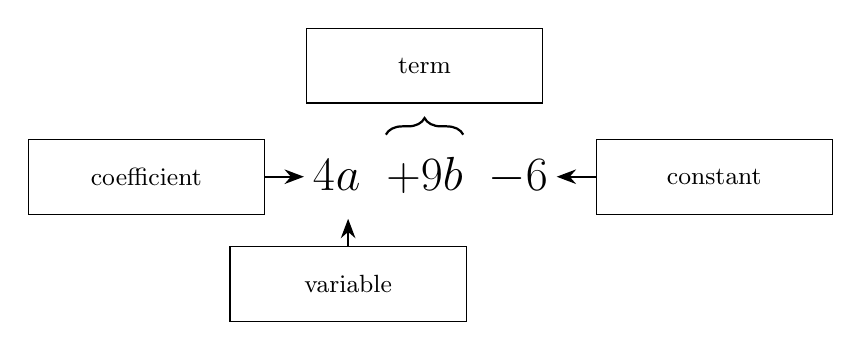
\begin{tikzpicture}[baseline=(a.base),
    namebox/.style={draw, minimum width=3.0cm, minimum height=0.95cm, inner sep=2pt}]
  \node[part] (c) {$4$};
  \node[part, anchor=base west] (a) at (c.base east) {$a$};
  \node[part, anchor=base west] (t) at ([xshift=9pt]a.base east) {$+9b$};
  \node[part, anchor=base west] (k) at ([xshift=9pt]t.base east) {$-6$};
  \node[namebox, anchor=east] (cl) at ([xshift=-0.6cm]c.west) {\small coefficient};
  \draw[arr] (cl.east) -- (c.west);
  \node[namebox, anchor=north] (al) at ([yshift=-0.45cm]a.south) {\small variable};
  \draw[arr] (al.north) -- (a.south);
  \draw[brc] (t.north west) -- (t.north east) coordinate[midway] (m);
  \node[namebox, anchor=south] at ([yshift=0.5cm]m) {\small term};
  \node[namebox, anchor=west] (kl) at ([xshift=0.6cm]k.east) {\small constant};
  \draw[arr] (kl.west) -- (k.east);
\end{tikzpicture}
\end{center}

\textbf{Solution:} The terms are \answer{\(4a\), \(+9b\) and \(-6\)}. The coefficient of \(a\) is \answer{\(4\)}; the variable in that term is \(a\). The term \answer{\(9b\)} is labelled as a term (its coefficient is \(9\) and its variable is \(b\)). The constant is \answer{\(-6\)}.
\end{solbox}

\vspace{6pt}
\parttitle{2}{Fill in the gaps}

\begin{solbox}
\textbf{Q3.} Consider \(4xy+2z-5\).

\begin{itemize}
  \item This expression has \answer{\(3\)} terms: \(4xy\), \(2z\) and \(-5\).
  \item Its \(3\) variables are \answer{\(x\), \(y\) and \(z\)}.
  \item The coefficient of the term \(xy\) is \answer{\(4\)}, because \(4xy\) means \(4\times xy\).
  \item The constant is \answer{\(-5\)}, because \(-5\) has no variable. The sign belongs to the term.
\end{itemize}
\end{solbox}

\begin{solbox}
\textbf{Q4.} Consider \(6m-n+8\).

\begin{itemize}
  \item The terms are \answer{\(6m\), \(-n\) and \(8\)}. The sign in front of \(n\) belongs to that term, so it is \(-n\), not \(n\).
  \item The coefficient of \(m\) is \answer{\(6\)}.
  \item The coefficient of \(n\) is \answer{\(-1\)}, because \(-n=-1\times n\).
  \item The \(8\) is called the \answer{constant}.
\end{itemize}
\end{solbox}

\begin{solbox}
\textbf{Q5.} An expression has variables \(p\) and \(q\). The coefficient of \(p\) is \(3\), the coefficient of \(q\) is \(-5\), and the constant is \(4\).

\begin{center}
  \answer{\(3p-5q+4\)}
\end{center}
(or any reordering, such as \(3p+4-5q\)). Explanation: \(3p\) has coefficient \(3\); \(-5q\) has coefficient \(-5\); \(4\) is the constant. The sign in front of \(5q\) belongs to the term, giving coefficient \(-5\).
\end{solbox}

\begin{solbox}
\textbf{Q6.} Write an expression with \(4\) terms, \(2\) variables and a constant of \(-1\).

One possible answer is
\begin{center}
  \answer{\(5a+2b+ab-1\)}
\end{center}
Its terms are \(5a\), \(2b\), \(ab\) and \(-1\): that is \(4\) terms. The variables are \(a\) and \(b\) (\(2\) variables). The constant is \(-1\). Many other answers are possible, for example \(3x+4y-xy-1\).
\end{solbox}

\end{document}